\ChapterImageStar[cap:revisionLiteratura]{Revisión sistemática de la literatura}{./images/fondo.png}\label{cap:revisionLiteratura}
% !TODO Insertar Taxonomía
\mbox{}\\
\section{Construcción de la bitácora}

En busca de una base teórica sólida para seleccionar un nuevo universo HTCondor y con el objetivo de tomar decisiones informadas, se llevó a cabo una revisión exhaustiva de la literatura existente sobre el tema. Este proceso se desarrolló en varias etapas:


\subsection{Planeación}

Esta etapa tuvo como objetivo definir el propósito general del \SMS (\textit{Systematic Mapping Study}), adoptando la metodología propuesta por \cite{Sepulveda2021}.
A su vez, definió aspectos como objetivos (ver cuadro~\ref{tab:metas}), preguntas de investigación (ver cuadro~\ref{tab:preguntas}) y métricas (ver cuadro~\ref{tab:metricas}). Para ello, se siguió el modelo
Objetivo-Pregunta-Métrica (\textit{goal-question-metric}, GQM).

\subsubsection{Definición de metas para el \SMS}

% Tabla METAS DEL SMS
\begin{table}[H]
	\centering
	\renewcommand{\arraystretch}{1.2} % Espaciado reducido
	\fontsize{9pt}{10pt}\selectfont % Tamaño de fuente 8pt
	\begin{tabular}{|p{1.5cm}|p{12.5cm}|}  % Total: 14cm
		\hline
		\textbf{Meta} & \textbf{Descripción}                                                                                                                                                                                                                                                                                                                                         \\ \hline
		G1            & Clasificar trabajos relacionados con los universos de HTCondor según su aplicación e impacto en los dominios de computación distribuida y paralela, HTC, desarrollo de Software, virtualización y microservicios, redes de computadoras, infraestructura computacional, inteligencia artificial, análisis de datos y pensamiento computacional, entre otros. \\ \hline
		G2            & Identificar y categorizar trabajos vinculados con los universos de HTCondor como herramienta para fortalecer funciones esenciales universitarias como: investigación, docencia, extensión e industria.                                                                                                                                                       \\ \hline
	\end{tabular}
	\caption{Definición de metas del SMS}
	\label{tab:metas}
\end{table}


\subsubsection{Definición de preguntas de investigación}\label{subsubsec:RQ-def}
%TABLA GOAL VS Preguntas
\begin{table}[H]
	\centering
	\renewcommand{\arraystretch}{1.2} % Espaciado reducido
	\fontsize{9pt}{10pt}\selectfont % Tamaño de fuente 8pt
	\begin{tabular}{|p{0.7cm}|p{1.3cm}|p{5.5cm}|p{6cm}|} % Total: 14cm
		\hline
		\textbf{Meta}                                                                                                                                                                                                                                                                                                                                    & \textbf{Pregunta} & \textbf{Descripción} & \textbf{Motivación}        \\ \hline

		G1                                                                                                                                                                                                                                                                                                                                               & Q1                &
		\textit{¿Qué trabajos relacionados con los universos de HTCondor tienen impacto en los dominios de computación distribuida y paralela, HTC, desarrollo de Software, virtualización y microservicios, redes de computadoras, infraestructura computacional, inteligencia artificial, análisis de datos y pensamiento computacional, entre otros?} &
		Sobre los universos de HTCondor que tienen impacto en los dominios de computación distribuida y paralela, \HTC, desarrollo de Software, virtualización y microservicios, redes de computadoras, infraestructura computacional, inteligencia artificial, análisis de datos, pensamiento computacional: 1 - Reconocer cómo están estructurados. 2 - Identificar sus aplicaciones. 3 - Determinar su motivación contextual. \\ \hline

		G2                                                                                                                                                                                                                                                                                                                                               & Q2                &
		\textit{¿Qué trabajos vinculados con los universos de HTCondor potencian las funciones esenciales universitarias como investigación, docencia, extensión e industria?}                                                                                                                                                                           &
		Sobre los universos de HTCondor que potencian las funciones sustantivas universitarias como investigación, docencia, extensión e industria: 1 - Reconocer cómo están estructurados. 2 - Identificar sus aplicaciones. 3 - Determinar su motivación contextual.                                                                                                                                                           \\ \hline
	\end{tabular}
	\caption{Definición de preguntas de investigación del SMS}
	\label{tab:preguntas}
\end{table}

\subsubsection{Definición de métricas}
%Tabla METRICAS
\begin{table}[H]
	\centering
	\renewcommand{\arraystretch}{1.2} % Menor espaciado entre filas
	\fontsize{9pt}{10pt}\selectfont % Tamaño de fuente 8pt
	\begin{tabular}{|c|p{13cm}|} % Total: 14cm
		\hline
		\textbf{Métrica} & \textbf{Descripción}                                                                                                                                                                                                                                                                                                                                                                                                                                                                                           \\ \hline
		M1               & Cantidad de trabajos relacionados con los Universos de HTCondor vinculados con los dominios de: Computación distribuida y paralela, HTC, Desarrollo de software, Tecnologías de virtualización y microservicios, Redes de computadores, Infraestructura computacional, Inteligencia artificial, Análisis de datos, Pensamiento computacional, entre otros. Y que además sean usados como herramienta para fortalecer funciones esenciales universitarias como: Investigación, Docencia, Extensión e Industria. \\ \hline
		M2               & Popularidad de cada Universo en los trabajos seleccionados.                                                                                                                                                                                                                                                                                                                                                                                                                                                    \\ \hline
		M3               & Porcentaje de trabajos seleccionados en la fase final respecto de la cantidad de trabajos iniciales.                                                                                                                                                                                                                                                                                                                                                                                                           \\ \hline
		M4               & Porcentaje de trabajos aportados por cada base de datos en el mapeo que se está desarrollando.                                                                                                                                                                                                                                                                                                                                                                                                                 \\ \hline
	\end{tabular}
	\caption{Definición de métricas del SMS}
	\label{tab:metricas}
\end{table}


\newpage \section{Búsqueda de estudios}


Esta etapa comprendió las siguientes secciones:
\begin{enumerate}
	\item Estrategia de búsqueda, ya sea independiente o combinada;
	\item Identificación general de estudios;
	\item Revisión de estudios; y finalmente,
	\item Selección de estudios para incluir en el SMS.\@
\end{enumerate}

\subsection{Estrategia de búsqueda}

Este trabajo combinó estrategias de búsqueda en bases de datos con la técnica de búsqueda en bola de nieve, lo que permitió ampliar y enriquecer la recopilación de estudios relevantes para el mapeo sistemático. Esta aproximación facilitó la identificación de investigaciones clave que podrían no haber sido detectadas mediante una búsqueda tradicional.

\subsection{Búsqueda en bases de datos}\label{subsec:busquedaBasesDatos}
Se seleccionaron las siguientes bases de datos para llevar a cabo el mapeo sistemático de estudios: ACM, IEEE Xplore, Springer, Taylor \& Francis y Science Direct. Estas fuentes fueron elegidas por su disponibilidad, relevancia y cobertura en el área de investigación, asegurando así la obtención de información actualizada y de calidad para el desarrollo del estudio.


\newpage
\subsubsection{Identificación de estudios mediante búsqueda en bases de datos}\label{subsubsec:identificacionEstudios}
En esta etapa del proceso fue necesario establecer un marco que ayudase a establecer las palabras clave más apropiadas para el mapeo sistemático de estudios para cada una de las bases de datos seleccionadas. Para ello se hizo uso del modelo PICOC (\textit{Population}, \textit{Intervention}, \textit{Comparator}, \textit{Outcome}, and \textit{Context}) como guía metodológica, sirviendo como herramienta de apoyo para este procedimiento. El resultado de este proceso puede verse en la tabla~\ref{table:modelo-picoc}

% TABLA modelo PICOC: Población - Intervención - Comparación  - Salida - Contexto
\begin{table}[H]
	\centering
	\renewcommand{\arraystretch}{1.5} % Espaciado reducido
	\fontsize{9pt}{10pt}\selectfont % Tamaño de fuente 8pt
	\begin{tabular}{|c|p{12cm}|} % Total: 14cm
		\hline
		\textbf{Componente} & \textbf{Descripción}                                                                                                                                                                                                                                                                                                                                                                                                                                                                             \\ \hline

		Población           & Trabajos relacionados con los universos de HTCondor según su aplicación e impacto en los dominios de computación distribuida y paralela, HTC, desarrollo de Software, virtualización y microservicios, redes de computadoras, infraestructura computacional, inteligencia artificial, análisis de datos, pensamiento computacional, entre otros. Que potencian las funciones sustantivas universitarias de investigación, docencia y extensión.                                                  \\ \hline

		Intervención        & Identificación y clasificación de un conjunto de trabajos relacionados con los universos de HTCondor según su aplicación e impacto en los dominios de computación distribuida y paralela, HTC, desarrollo de Software, virtualización y microservicios, redes de computadoras, infraestructura computacional, inteligencia artificial, análisis de datos, pensamiento computacional, entre otros. Que potencian las funciones sustantivas universitarias de investigación, docencia y extensión. \\ \hline

		Comparación         &
		\textbf{1.} Casos de proyecto documentados.
		\textbf{2.} Cumplimiento de criterios de inclusión y exclusión.
		\textbf{3.} Aparición en bases de datos seleccionadas.                                                                                                                                                                                                                                                                                                                                                                                                                                                                 \\ \hline
		Salida              & Taxonomía que organiza los trabajos relacionados con los universos de HTCondor según su aplicación e impacto en los dominios de computación distribuida y paralela, HTC, desarrollo de Software, virtualización y microservicios, redes de computadoras, infraestructura computacional, inteligencia artificial, análisis de datos, pensamiento computacional, entre otros. Que potencian las funciones sustantivas universitarias de investigación, docencia y extensión.                       \\ \hline
		Contexto            & Universos HTCondor en dominios de computación distribuida y paralela, HTC, desarrollo de Software, virtualización y microservicios, redes de computadoras, infraestructura computacional, inteligencia artificial, análisis de datos, pensamiento computacional, entre otros. Que potencian las funciones sustantivas universitarias de investigación, docencia y extensión.                                                                                                                     \\ \hline
	\end{tabular}
	\caption{Modelo PICOC}
	\label{table:modelo-picoc}
\end{table}



%# TABLA Palabras clave indentificadas usando el modelo PICOC.
\begin{table}[H]
	\centering
	\renewcommand{\arraystretch}{1.4}
	\fontsize{8}{8}\selectfont
	\begin{tabular}{|p{3cm}|p{10.0cm}|}
		\hline
		\textbf{Categoría \hbox{PICOC}} & \textbf{Palabras clave} \\
		\hline
		Población                       &
		- Trabajos relacionados \newline
		- Universos \newline
		- HTCondor \newline
		- Computación distribuida y paralela \newline
		- HTC \newline
		- Desarrollo de Software \newline
		- Virtualización y microservicios \newline
		- Redes de computadoras \newline
		- Infraestructura computacional \newline
		- Inteligencia artificial \newline
		- Análisis de datos \newline
		- Pensamiento computacional \newline
		- Investigación \newline
		- Docencia \newline
		- Extensión                                               \\
		\hline
		Intervención                    &
		- Identificación \newline
		- Clasificación \newline
		- Universos \newline
		- HTCondor \newline
		- Computación distribuida y paralela \newline
		- HTC \newline
		- Desarrollo de Software \newline
		- Virtualización y microservicios \newline
		- Redes de computadoras \newline
		- Infraestructura computacional \newline
		- Inteligencia artificial \newline
		- Análisis de datos \newline
		- Pensamiento computacional \newline
		- Investigación \newline
		- Docencia \newline
		- Extensión                                               \\
		\hline
		Criterios de aceptación         &
		- Casos de estudio culminados                             \\
		\hline
		Salidas                         &
		- Taxonomía \newline
		- Universos \newline
		- HTCondor \newline
		- Computación distribuida y paralela \newline
		- HTC \newline
		- Desarrollo de Software \newline
		- Virtualización y microservicios \newline
		- Redes de computadoras \newline
		- Infraestructura computacional \newline
		- Inteligencia artificial \newline
		- Análisis de datos \newline
		- Pensamiento computacional \newline
		- Investigación \newline
		- Docencia \newline
		- Extensión                                               \\
		\hline
		Contexto                        &
		- Universos \newline
		- HTCondor \newline
		- Computación distribuida y paralela \newline
		- HTC \newline
		- Desarrollo de Software \newline
		- Virtualización y microservicios \newline
		- Redes de computadoras \newline
		- Infraestructura computacional \newline
		- Inteligencia artificial \newline
		- Análisis de datos \newline
		- Pensamiento computacional \newline
		- Investigación \newline
		- Docencia \newline
		- Extensión                                               \\
		\hline
	\end{tabular}
	\caption{Palabras clave identificadas usando el modelo PICOC}
	\label{table:keywords-picoc}
\end{table}

Las palabras clave identificadas en el cuadro~\ref{table:keywords-picoc} se complementaron con sinónimos y términos relacionados, los cuales se presentan en el cuadro~\ref{tab:keywords}. Estas keywords se utilizaron para construir las cadenas de búsqueda en cada base de datos.


%# TABLA Keywoords para las cadenas de búsqueda,
\begin{table}[H]
	\centering
	\scriptsize
	\setlength{\tabcolsep}{4pt}
	\fontsize{9pt}{10pt}\selectfont % Tamaño de fuente 8pt
	\begin{tabular}{|c|p{12.5cm}|} % Total: 14cm
		\hline
		\textbf{Palabras clave} & \textbf{Sinónimos}                                                             \\
		\hline
		HTCondor                & High Throughput Condor, Distributed Computing Framework, Condor                \\
		\hline
		HTC                     & HPC, High Throughput Computing, High Performance Computing                     \\
		\hline
		Universe                & Execution Environment, Runtime Environment, Cluster                            \\
		\hline
		Project                 & Work, Implementation, Implement, Deployment, Development, Program, Plan, Study \\
		\hline
		Research                & Teaching, Extension, Outreach, Industry                                        \\
		\hline
	\end{tabular}
	\caption{Palabras clave para la búsqueda en base de datos}
	\label{tab:keywords}
\end{table}



\noindent
Con el objetivo de filtrar los resultados y enfocarse en estudios relevantes, se definieron criterios de inclusión y exclusión, los cuales se presentan en el cuadro~\ref{table:criterios-inclusion-exclusion}. Estos criterios ayudaron a seleccionar artículos que se alinean con los objetivos del \SMS y a descartar aquellos que no aportan valor al análisis.

% TABLA Criterios de inclusión y exclusión
\begin{table}[H]
	\centering
	\caption{Criterios de inclusión y exclusión}
	\fontsize{9pt}{10pt}\selectfont % Tamaño de fuente 8pt
	\begin{tabular}{|p{3cm}|p{5cm}|p{6cm}|}
		\hline
		\textbf{Categoría}  & \textbf{Inclusión}         & \textbf{Exclusión}                                                                                                          \\
		\hline
		Tipo de publicación & Artículos de investigación & Tesis, capítulos de libros, libros, revistas, conferencias, y todo lo demás que no esté en el tipo de publicación inclusiva \\
		\hline
		Período             & Desde 2020 hasta 2024      & -                                                                                                                           \\
		\hline
		Idioma              & Inglés                     & -                                                                                                                           \\
		\hline
	\end{tabular}
	\label{table:criterios-inclusion-exclusion}
\end{table}



%##################
%##################
%##################
%##################
%##################




\subsubsection{Búsqueda en bases de datos}\label{par:busquedaBasesDatos}
\noindent
Las cadenas de búsqueda específicas para cada base de datos se encuentran en la sección~\ref{sec:cadenas-busqueda} del apéndice.

\subsubsection{Métricas de la búsqueda sin criterios de inclusión/exclusión}\label{subsubsec:resumenBusqueda}
\noindent
La Tabla~\ref{table:bases-sin-exclusion} presenta el número de publicaciones identificadas en las principales bases de datos consultadas durante la revisión inicial de literatura, antes de aplicar los criterios de inclusión y exclusión. En total se recuperaron 847 registros, distribuidos de la siguiente manera: ACM (518), IEEE (0), Springer (209), Science Direct (120) y Taylor \& Francis (0). Estos resultados se evidencian en el apéndice~\ref{sec:busqueda-sin-criterios}.

% TABLA Resultados de busqueda sin exclusión
\begin{table}[H]
	\centering
	\caption{Resultados de las cadenas de búsqueda}
	\label{table:bases-sin-exclusion}
	\fontsize{8pt}{10pt}\selectfont % Tamaño de fuente 8pt
	\begin{tabular}{|p{3.5cm}|>{\centering\arraybackslash}p{1.0cm}|>{\centering\arraybackslash}p{1.0cm}|>{\centering\arraybackslash}p{2.0cm}|>{\centering\arraybackslash}p{1.3cm}|>{\centering\arraybackslash}p{2.3cm}|>{\centering\arraybackslash}p{1.0cm}|}
		\hline
		\textbf{Criterios}                               & \textbf{ACM} & \textbf{IEEE} & \textbf{ScienceDirect} & \textbf{Springer} & \textbf{Taylor\&Francis} & \textbf{Total} \\
		\hline
		Cadena de búsqueda con palabras clave únicamente & 518          & 0             & 120                    & 209               & 0                        & 847            \\
		\hline
		Contribución porcentual                          & 61.16\%      & 0\%           & 14.17\%                & 24.68\%           & 0\%                      & 100\%          \\
		\hline
	\end{tabular}
\end{table}





\subsubsection{Métricas de la búsqueda con criterios de inclusión/exclusión}\label{subsec:resumenBusquedaCriterios}
\noindent
Esta búsqueda se realizó considerando los criterios de exclusión e inclusión definidos previamente. Las cadenas de búsqueda son exactamente iguales que antes, este punto se diferencia por la aplicación de filtros. Para ver las capturas de pantalla veáse el apéndice~\ref{sec:busqueda-con-criterios}.
La Tabla~\ref{table:bases-con-exclusion} muestra los resultados obtenidos tras aplicar los criterios de inclusión y exclusión previamente definidos. A diferencia de la búsqueda inicial, en esta fase se utilizaron filtros específicos que redujeron significativamente la cantidad de publicaciones relevantes. En total se identificaron 976 documentos, distribuidos en las bases de datos de la siguiente manera: ACM (48), IEEE (134), Springer (592), Science Direct (46) y Taylor \& Francis (156).

% TABLA Bases de datos con inclusión
\begin{table}[H]
	\centering
	\caption{Resultados de las cadenas de búsqueda con criterios de exclusión}
	\label{table:bases-con-exclusion}
	\fontsize{8pt}{10pt}\selectfont % Tamaño de fuente 8pt
	\begin{tabular}{|p{3.5cm}|>{\centering\arraybackslash}p{1.0cm}|>{\centering\arraybackslash}p{1.0cm}|>{\centering\arraybackslash}p{2.0cm}|>{\centering\arraybackslash}p{1.3cm}|>{\centering\arraybackslash}p{2.3cm}|>{\centering\arraybackslash}p{1.0cm}|}
		\hline
		\textbf{Criterios}                               & \textbf{ACM} & \textbf{IEEE} & \textbf{ScienceDirect} & \textbf{Springer} & \textbf{Taylor \& Francis} & \textbf{Total} \\
		\hline
		Cadena de búsqueda con palabras clave únicamente & 315          & 0             & 101                    & 63                & 0                          & 479            \\
		\hline
		Contribución porcentual                          & 65.76\%      & 0\%           & 21.09\%                & 13.15\%           & 0\%                        & 100\%          \\
		\hline
	\end{tabular}
\end{table}

El fruto del proceso logrado en la búsqueda de bases de datos puede verse en la figura \ref{fig:resumen-busqueda-bases-de-datos}. Como se puede observar, luego de aplicación de los criterios de exclusión, se perdieron 368 estudios, un perdida porcentual del 43.44\% respecto los resultados de la búsqueda inicial.

% FIGURA de resultados de ambos procesos de busqueda con y sin criterios.
\begin{figure}[H]
	\centering
	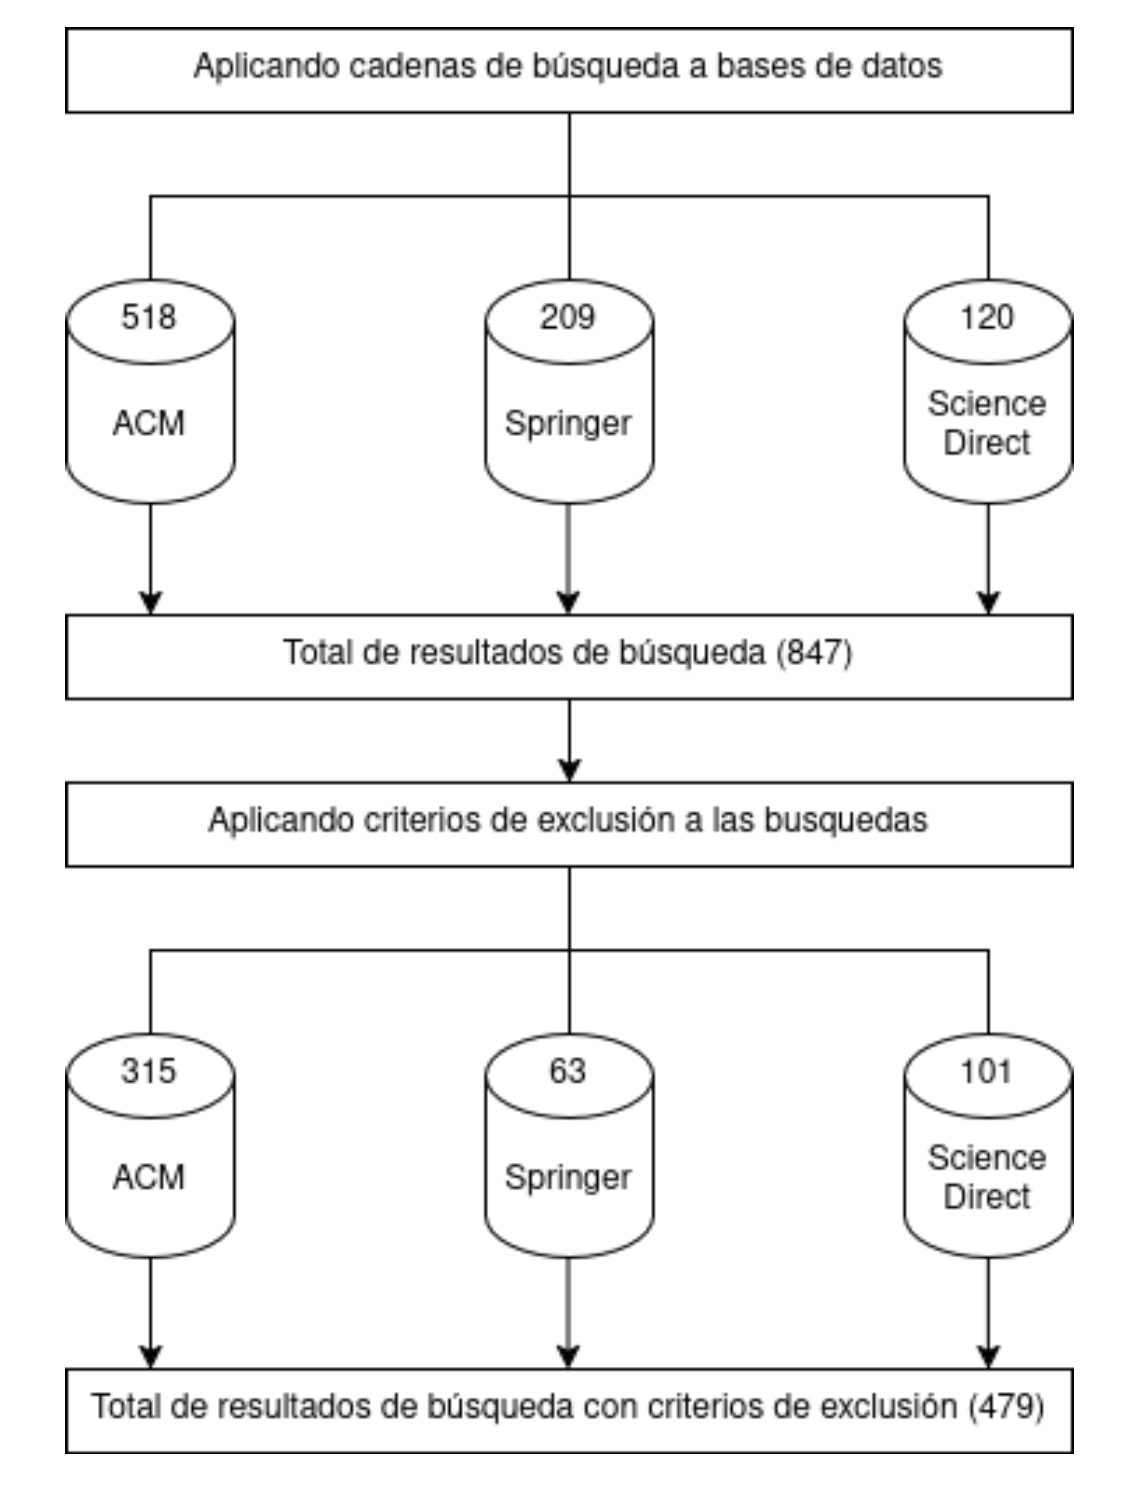
\includegraphics[scale=0.6] {tablas-images/sms/resumen_busqueda_bases.png}
	\caption{Diagrama resumen del proceso de búsqueda en bases de datos}\label{fig:resumen-busqueda-bases-de-datos}
\end{figure}




\section{Eliminación de duplicados}\label{sec:eliminacionDuplicados}
\noindent
La eliminación de estudios duplicados se efectuó mediante la herramienta de gestión bibliográfica Mendeley. Tras la recopilación inicial, todos los artículos fueron importados a dicha plataforma, la cual identificó y eliminó automáticamente las publicaciones redundantes. Este proceso resultó en la exclusión de \textbf{tres} artículos duplicados, reduciendo el total de estudio a 476. La figura \ref{fig:eliminacion-duplicados} presenta una visualización gráfica de estos resultados.


% FIGURA Eliminación de duplicados
\begin{figure}[H]
	\centering
	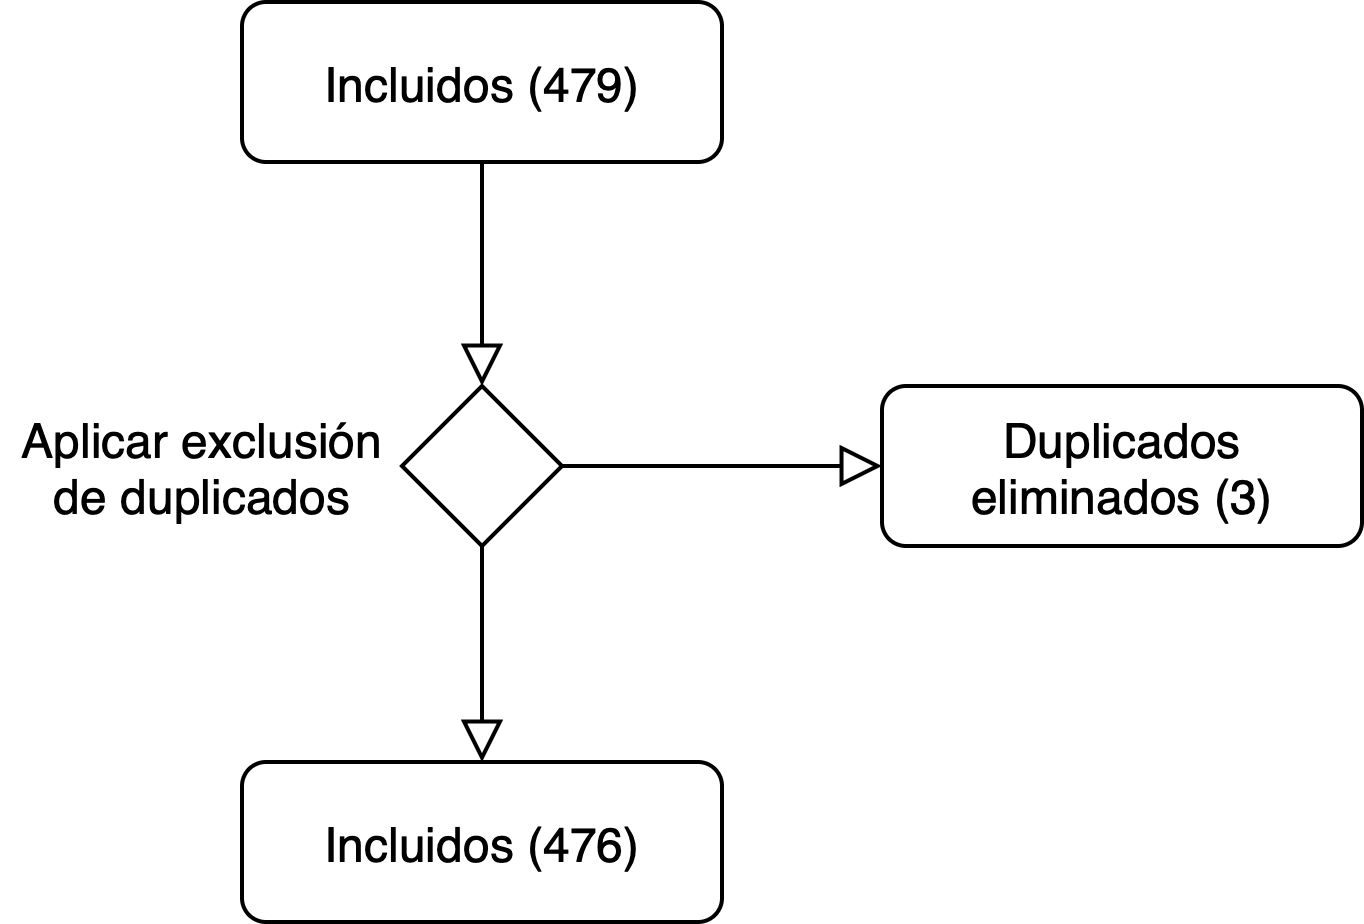
\includegraphics[scale=0.25] {tablas-images/sms/eliminacion-duplicados.png}
	\caption{Diagrama del proceso de eliminación de resultados}\label{fig:eliminacion-duplicados}
\end{figure}


\section{Priorización de estudios}\label{sec:priorizacionEstudios}
\noindent


Luego de la selección inicial de los artículos, se procedió a examinar los campos  \textit{title}, \textit{abstract} y \textit{keywords} de cada uno. Como resultado de esta revisión se generaron métricas de calidad para cada artículo, con el fin de priorizar aquellos más relevantes para la investigación. Las métricas utilizadas fueron las siguientes:

\begin{itemize}
	\item \textbf{SCI} \textit{(Science Citation Index)}
	\item \textbf{CVI} \textit{(Core Value Index)}
	\item \textbf{IRRQ} \textit{(Index Relation Research Question)}
\end{itemize}
\noindent

Este proceso inició con un total de 476 artículos, los cuales fueron evaluados según su alineamiento con los objetivos de la investigación. La evaluación temática permitió identificar un total de 99 artículos con una relación directa con el enfoque planteado.

\section{Estrategia de búsqueda usando bola de nieve}\label{sec:bolaDeNieve}
\noindent

En esta etapa, se seleccionó el primer cuartil según el índice \SCI, obteniendo un total de 24 artículos que constituyeron la línea base para el proceso de búsqueda por bola de nieve. A partir de esta base, se aplicó la estrategia de bola de nieve en ambas direcciones: hacia adelante (revisando referencias citadas por los artículos base) y hacia atrás (identificando artículos que citan a los de la base). En la primera iteración se obtuvieron tres artículos mediante la técnica hacia atrás y cuatro mediante la técnica hacia adelante. La segunda iteración produjo tres artículos adicionales con bola de nieve hacia atrás y cinco con bola de nieve hacia adelante. En total, el proceso de bola de nieve generó 15 artículos adicionales. Sumando estos resultados a los 99 artículos previamente filtrados por \SCI, se obtuvo un corpus final de 114 artículos para el análisis.

El resumen de este proceso puede verse en la figura \ref{fig:resumen-snowball}

\begin{figure}[H]
	\begin{center}
		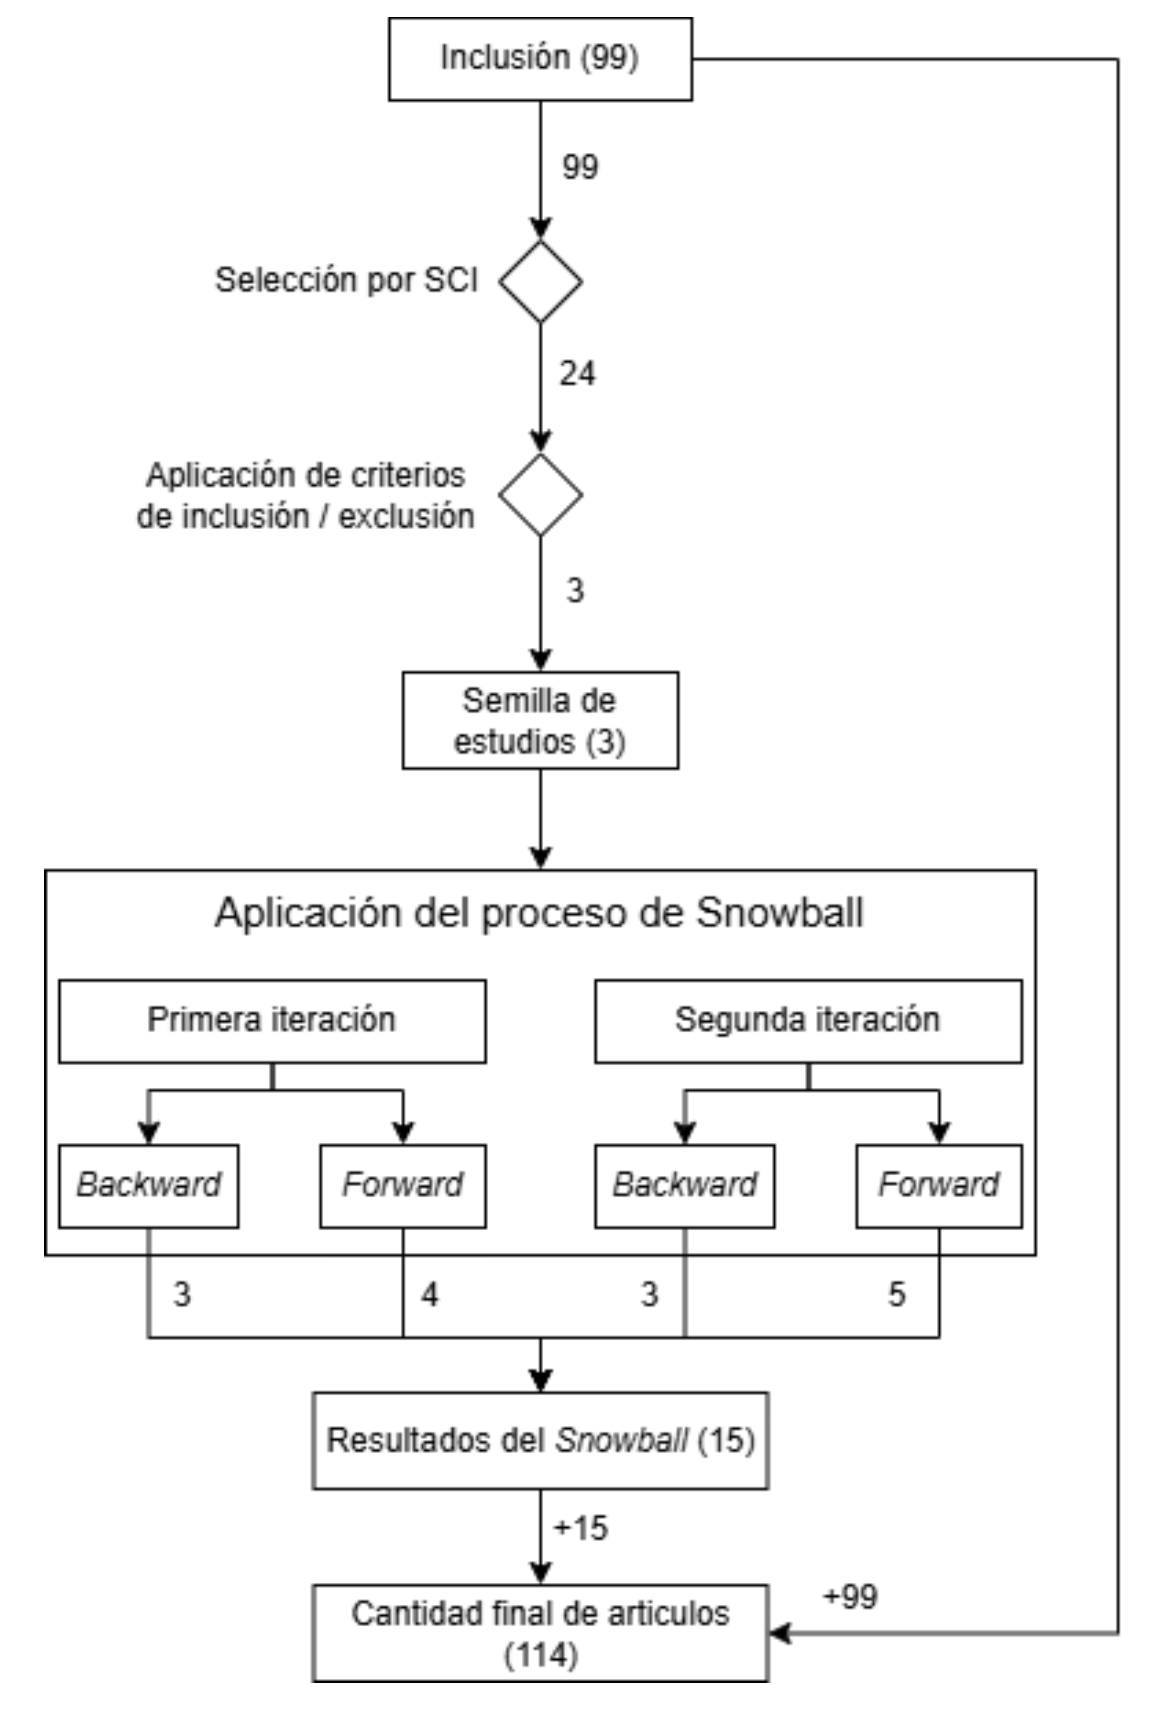
\includegraphics[width=0.6\textwidth]{tablas-images/sms/resumen-snowball.png}
	\end{center}
	\caption{}\label{fig:resumen-snowball}
\end{figure}


\section{Identificación de estudios}

\section{Cuadro de estudios}

Los estudios resultantes del proceso de \SMS se presentan en la tabla \ref{table:selected_primary_studies}.



% -------- Tabla : Estudios Primarios Seleccionados (SPSs) ------------
\begin{table}[H]
	\centering
	\caption{Los 114 estudios primarios seleccionados (SPSs)}
	\label{table:selected_primary_studies}
	\fontsize{8pt}{10pt}\selectfont % Tamaño de fuente 8pt
	\renewcommand{\arraystretch}{1.2}
	\begin{tabular*}{\textwidth}{l @{\extracolsep{\fill}} r l @{\extracolsep{\fill}} r l @{\extracolsep{\fill}} r l @{\extracolsep{\fill}} r l @{\extracolsep{\fill}} r}
		\toprule
		\textbf{ID} & \textbf{Ref}                        & \textbf{ID} & \textbf{Ref}                        & \textbf{ID} & \textbf{Ref}                      & \textbf{ID} & \textbf{Ref}                        & \textbf{ID} & \textbf{Ref}                       \\
		\midrule
		SPS001      & \spsone                             & SPS002      & \spstwo                             & SPS003      & \spsthree                         & SPS004      & \spsfour                            & SPS005      & \spsfive                           \\
		SPS006      & \spssix                             & SPS007      & \spsseven                           & SPS008      & \spseight                         & SPS009      & \spsnine                            & SPS010      & \spsten                            \\
		SPS011      & \spseleven                          & SPS012      & \spstwelve                          & SPS013      & \spsthirteen                      & SPS014      & \spsfourteen                        & SPS015      & \spsfifteen                        \\
		SPS016      & \spssixteen                         & SPS017      & \spsseventeen                       & SPS018      & \spseighteen                      & SPS019      & \spsnineteen                        & SPS020      & \spstwenty                         \\
		SPS021      & \spstwentyone                       & SPS022      & \spstwentytwo                       & SPS023      & \spstwentythree                   & SPS024      & \spstwentyfour                      & SPS025      & \spstwentyfive                     \\
		SPS026      & \spstwentysix                       & SPS027      & \spstwentyseven                     & SPS028      & \spstwentyeight                   & SPS029      & \spstwentynine                      & SPS030      & \spsthirty                         \\
		SPS031      & \spsthirtyone                       & SPS032      & \spsthirtytwo                       & SPS033      & \spsthirtythree                   & SPS034      & \spsthirtyfour                      & SPS035      & \spsthirtyfive                     \\
		SPS036      & \spsthirtysix                       & SPS037      & \spsthirtyseven                     & SPS038      & \spsthirtyeight                   & SPS039      & \spsthirtynine                      & SPS040      & \spsforty                          \\
		SPS041      & \spsfortyone                        & SPS042      & \spsfortytwo                        & SPS043      & \spsfortythree                    & SPS044      & \spsfortyfour                       & SPS045      & \spsfortyfive                      \\
		SPS046      & \spsfortysix                        & SPS047      & \spsfortyseven                      & SPS048      & \spsfortyeight                    & SPS049      & \spsfortynine                       & SPS050      & \spsfifty                          \\
		SPS051      & \spsfiftyone                        & SPS052      & \spsfiftytwo                        & SPS053      & \spsfiftythree                    & SPS054      & \spsfiftyfour                       & SPS055      & \spsfiftyfive                      \\
		SPS056      & \spsfiftysix                        & SPS057      & \spsfiftyseven                      & SPS058      & \spsfiftyeight                    & SPS059      & \spsfiftynine                       & SPS060      & \spssixty                          \\
		SPS061      & \spssixtyone                        & SPS062      & \spssixtytwo                        & SPS063      & \spssixtythree                    & SPS064      & \spssixtyfour                       & SPS065      & \spssixtyfive                      \\
		SPS066      & \spssixtysix                        & SPS067      & \spssixtyseven                      & SPS068      & \spsixtyeight                     & SPS069      & \spssixtynine                       & SPS070      & \spsseventy                        \\
		SPS071      & \spsseventyone                      & SPS072      & \spsseventytwo                      & SPS073      & \spsseventythree                  & SPS074      & \spsseventyfour                     & SPS075      & \spsseventyfive                    \\
		SPS076      & \spsseventysix                      & SPS077      & \spsseventyseven                    & SPS078      & \spsseventyeight                  & SPS079      & \spsseventynine                     & SPS080      & \spseighty                         \\
		SPS081      & \spseightyone                       & SPS082      & \spseightytwo                       & SPS083      & \spseightythree                   & SPS084      & \spseightyfour                      & SPS085      & \spseightyfive                     \\
		SPS086      & \spseightysix                       & SPS087      & \spseightyseven                     & SPS088      & \spseightyeight                   & SPS089      & \spseightynine                      & SPS090      & \spsninety                         \\
		SPS091      & \spsninetyone                       & SPS092      & \spsninetytwo                       & SPS093      & \spsninetythree                   & SPS094      & \spsninetyfour                      & SPS095      & \spsninetyfive                     \\
		SPS096      & \spsninetysix                       & SPS097      & \spsninetyseven                     & SPS098      & \spsnineyeight                    & SPS099      & \spsninetynine                      & SPS100      & \spsonehundred                     \\
		SPS101      & \spsonehundredone                   & SPS102      & \spsonehundredtwo                   & SPS103      & \spsonehundredthree               & SPS104      & \spsonehundredfour                  & SPS105      & \spsonehundredfive                 \\
		SPS106      & \spsonehundredsix                   & SPS107      & \spsonehundredseven                 & SPS108      & \spsonehundredeight               & SPS109      & \spsonehundrednine                  & SPS110      & \spsonehundredten                  \\
		SPS111      & \spsonehundredeleven                & SPS112      & \spsonehundredtwelve                & SPS113      & \spsonehundredthirteen            & SPS114      & \spsonehundredfourteen              &             &                                    \\
		\bottomrule
	\end{tabular*}
	\vspace{5pt}
\end{table}

%  --------------------------------------------------------------


\subsection{Artículos por año y métricas}
\noindent
A continuación se presentan las gráficas de los resultados de la búsqueda. En la figura \ref{fig:plot-anios-vs-indices-calidad} se muestra la relación entre la cantidad de estudios por año y las métricas definidas en las sección \ref{sec:priorizacionEstudios}

\begin{figure}[H]
	\begin{center}
		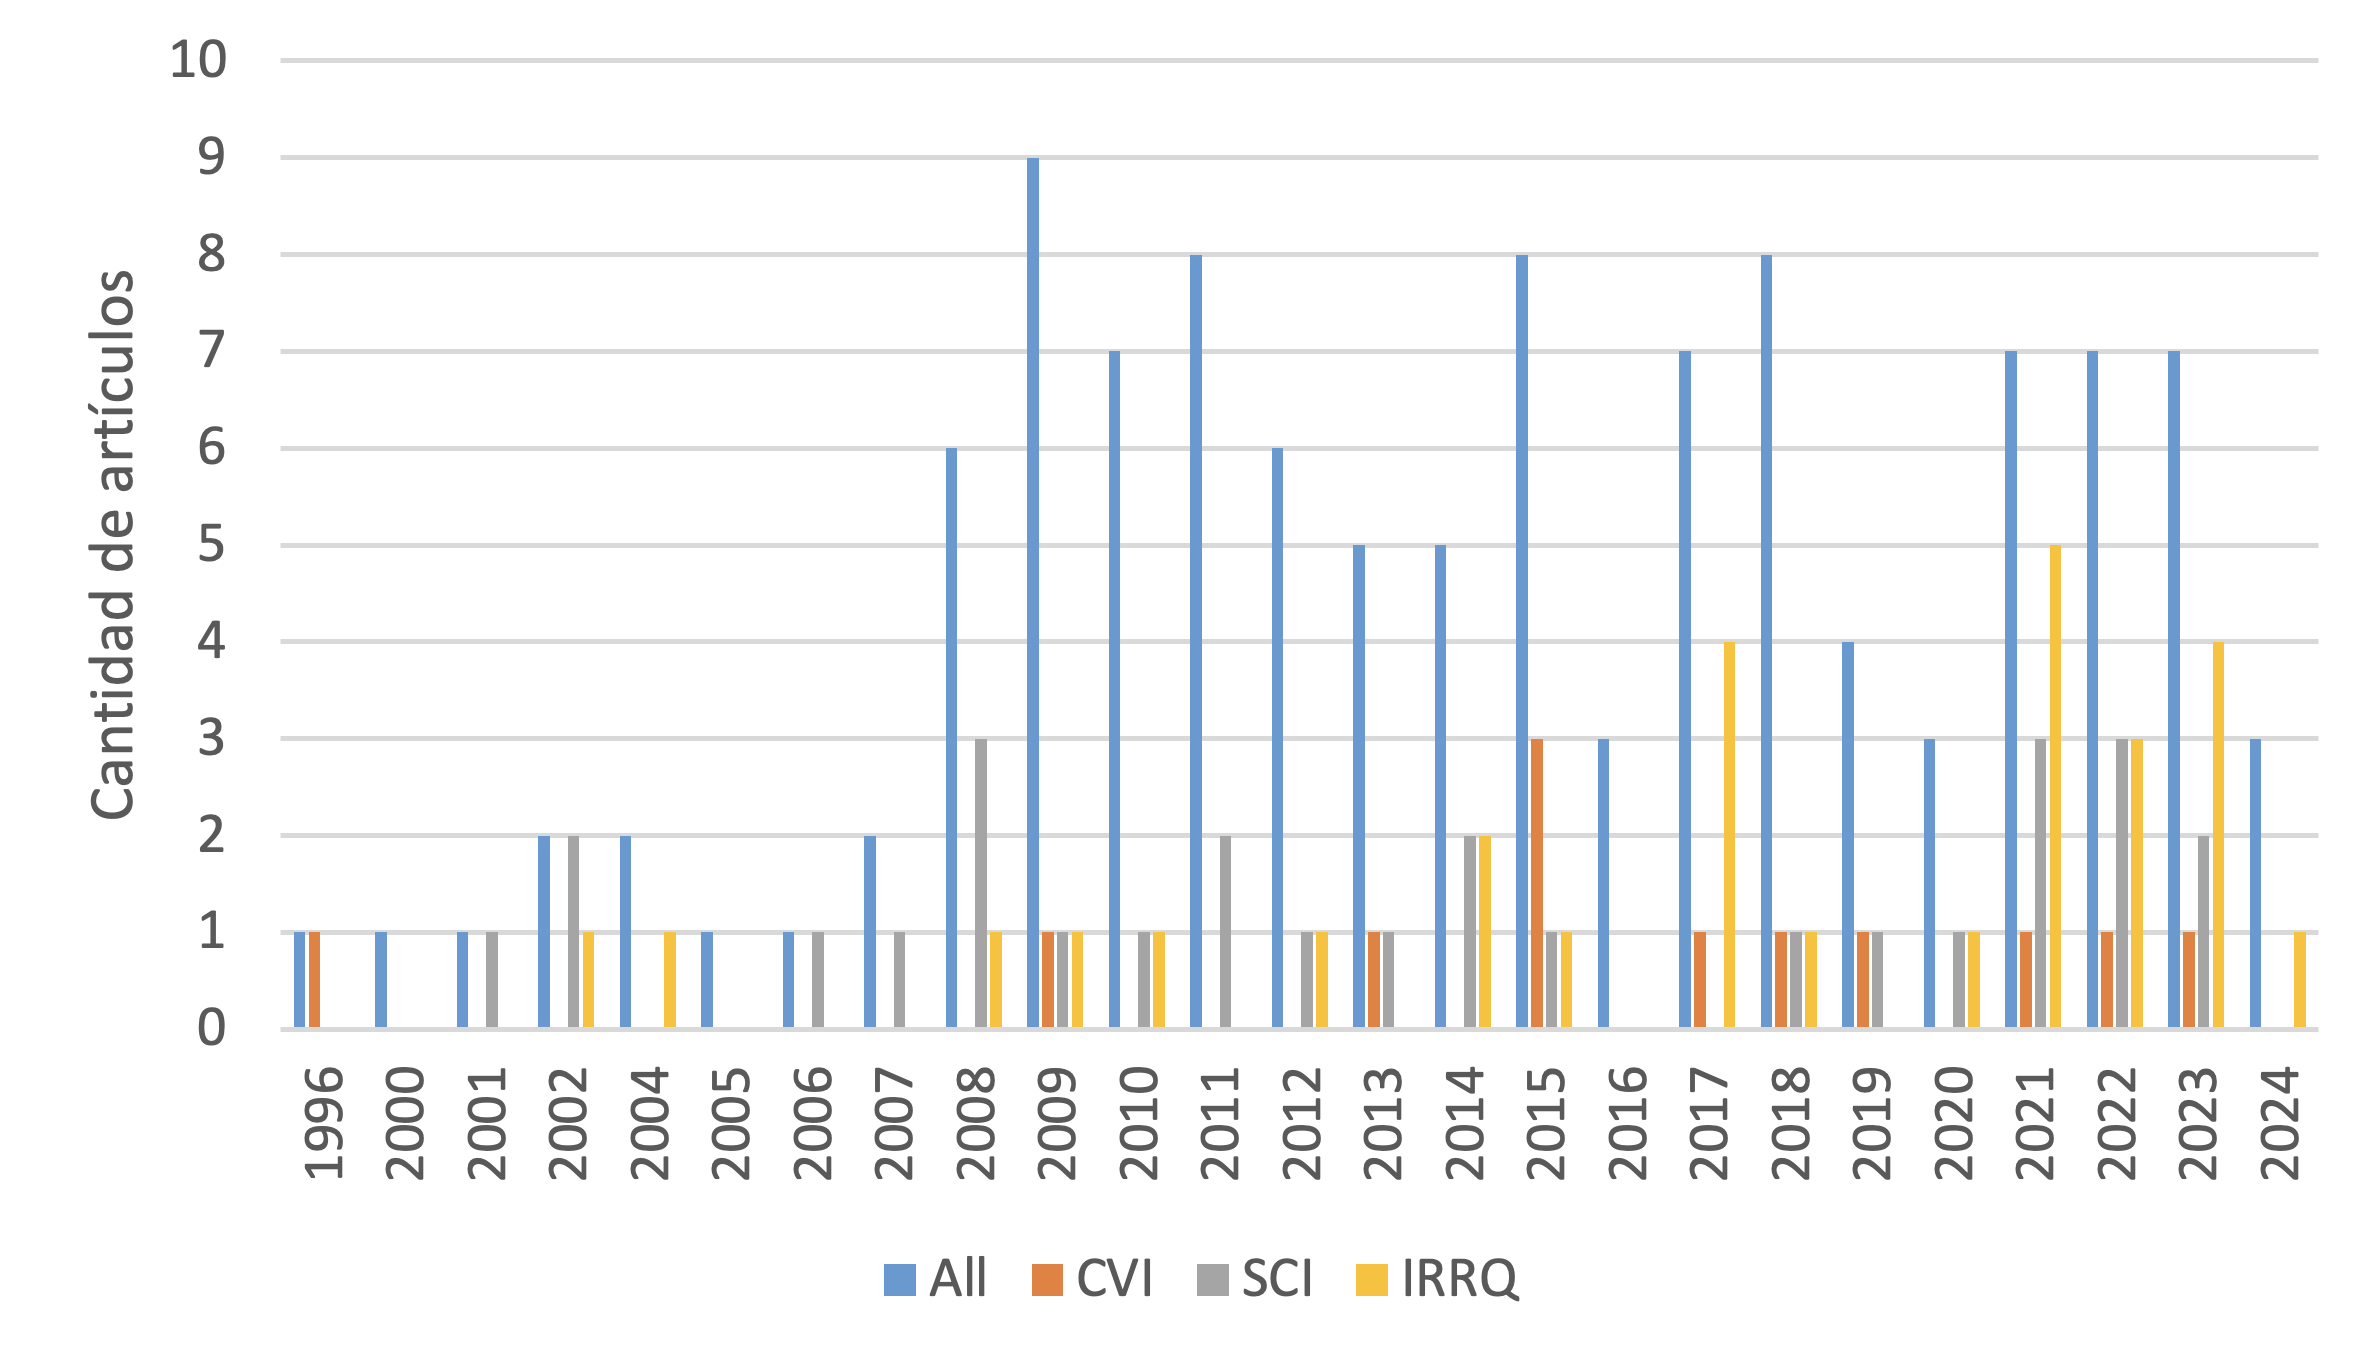
\includegraphics[width=0.95\textwidth]{tablas-images/sms/plot-freq-indices.png}
	\end{center}
	\caption{Cantidad de artículos en conformodidad con las métricas de calidad definidas en \ref{sec:priorizacionEstudios}}
	\label{fig:plot-anios-vs-indices-calidad}
\end{figure}



\subsection{Diferencias entre estrategias}

En la figura \ref{fig:plot-estrategia_vs_articulos} se pude apreciar la cantidad de artículos obtenido por cada

\begin{figure}[H]
	\centering
	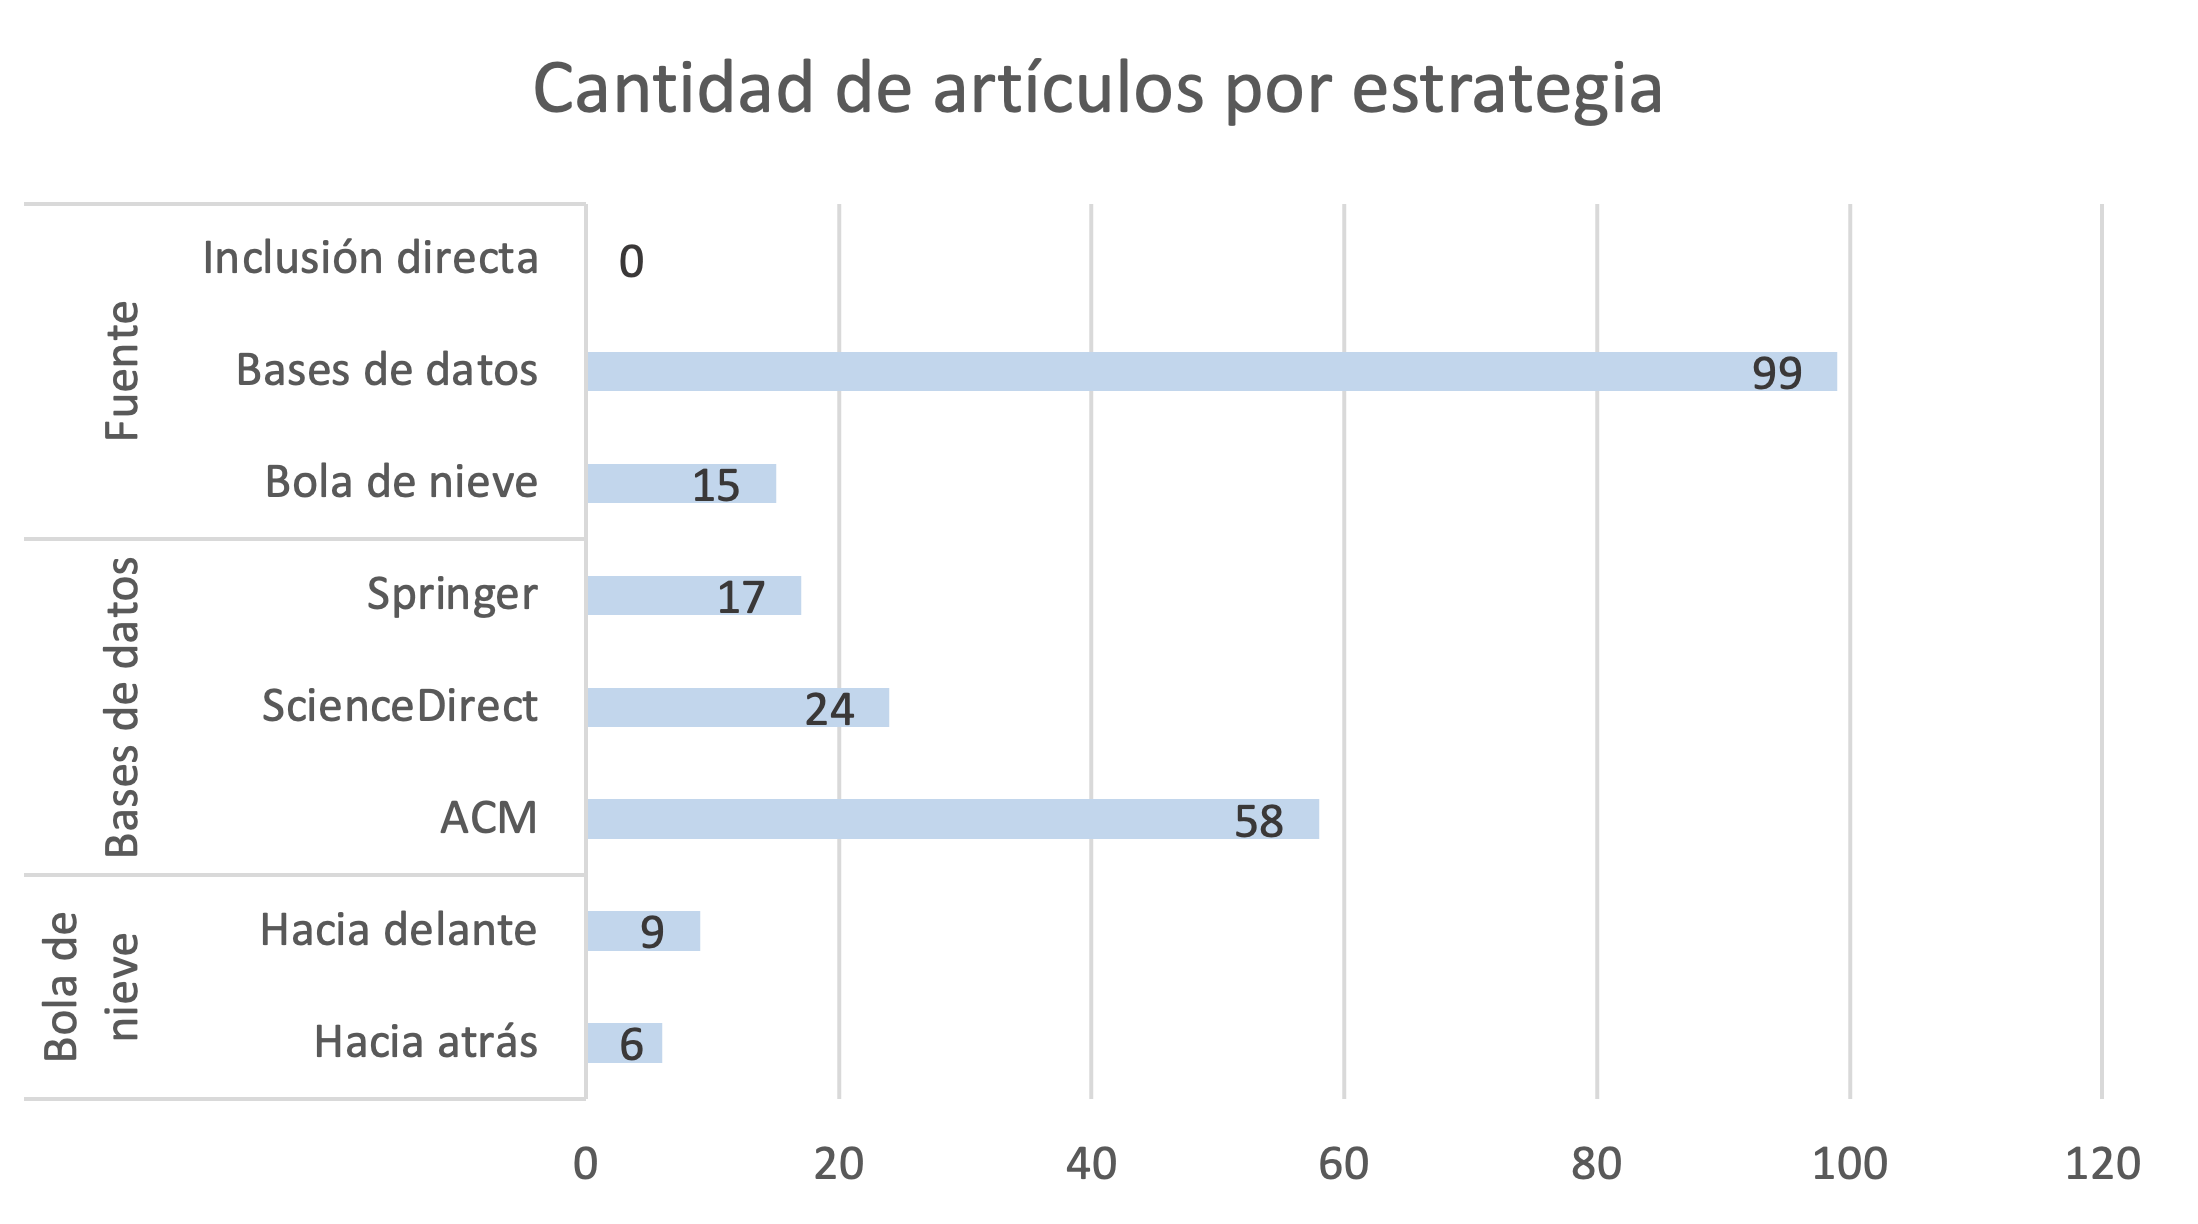
\includegraphics[scale=0.3] {tablas-images/sms/plot-estrategia_vs_articulos.png}
	\caption{Diagrama del proceso de eliminación de resultados}\label{fig:plot-estrategia_vs_articulos}
\end{figure}

\subsection{Tópicos frecuentes en los estudios}
\noindent

Del conjunto de 114 estudios analizados, se identificaron tópicos recurrentes mediante el análisis sistemático de los~\textit{abstracts} y~\textit{keywords} de cada publicación. Esta categorización temática reveló las áreas de investigación predominantes en el campo de estudio. Como se ilustra en la figura~\ref{fig:plot-topicos}, los tópicos más frecuentes incluyen \textbf{Grid Computing, \HPC, Cloud Computing, \HTC, y Parallel}, los cuales representan las tendencias principales en la literatura analizada.

\begin{figure}[H]
	\centering
	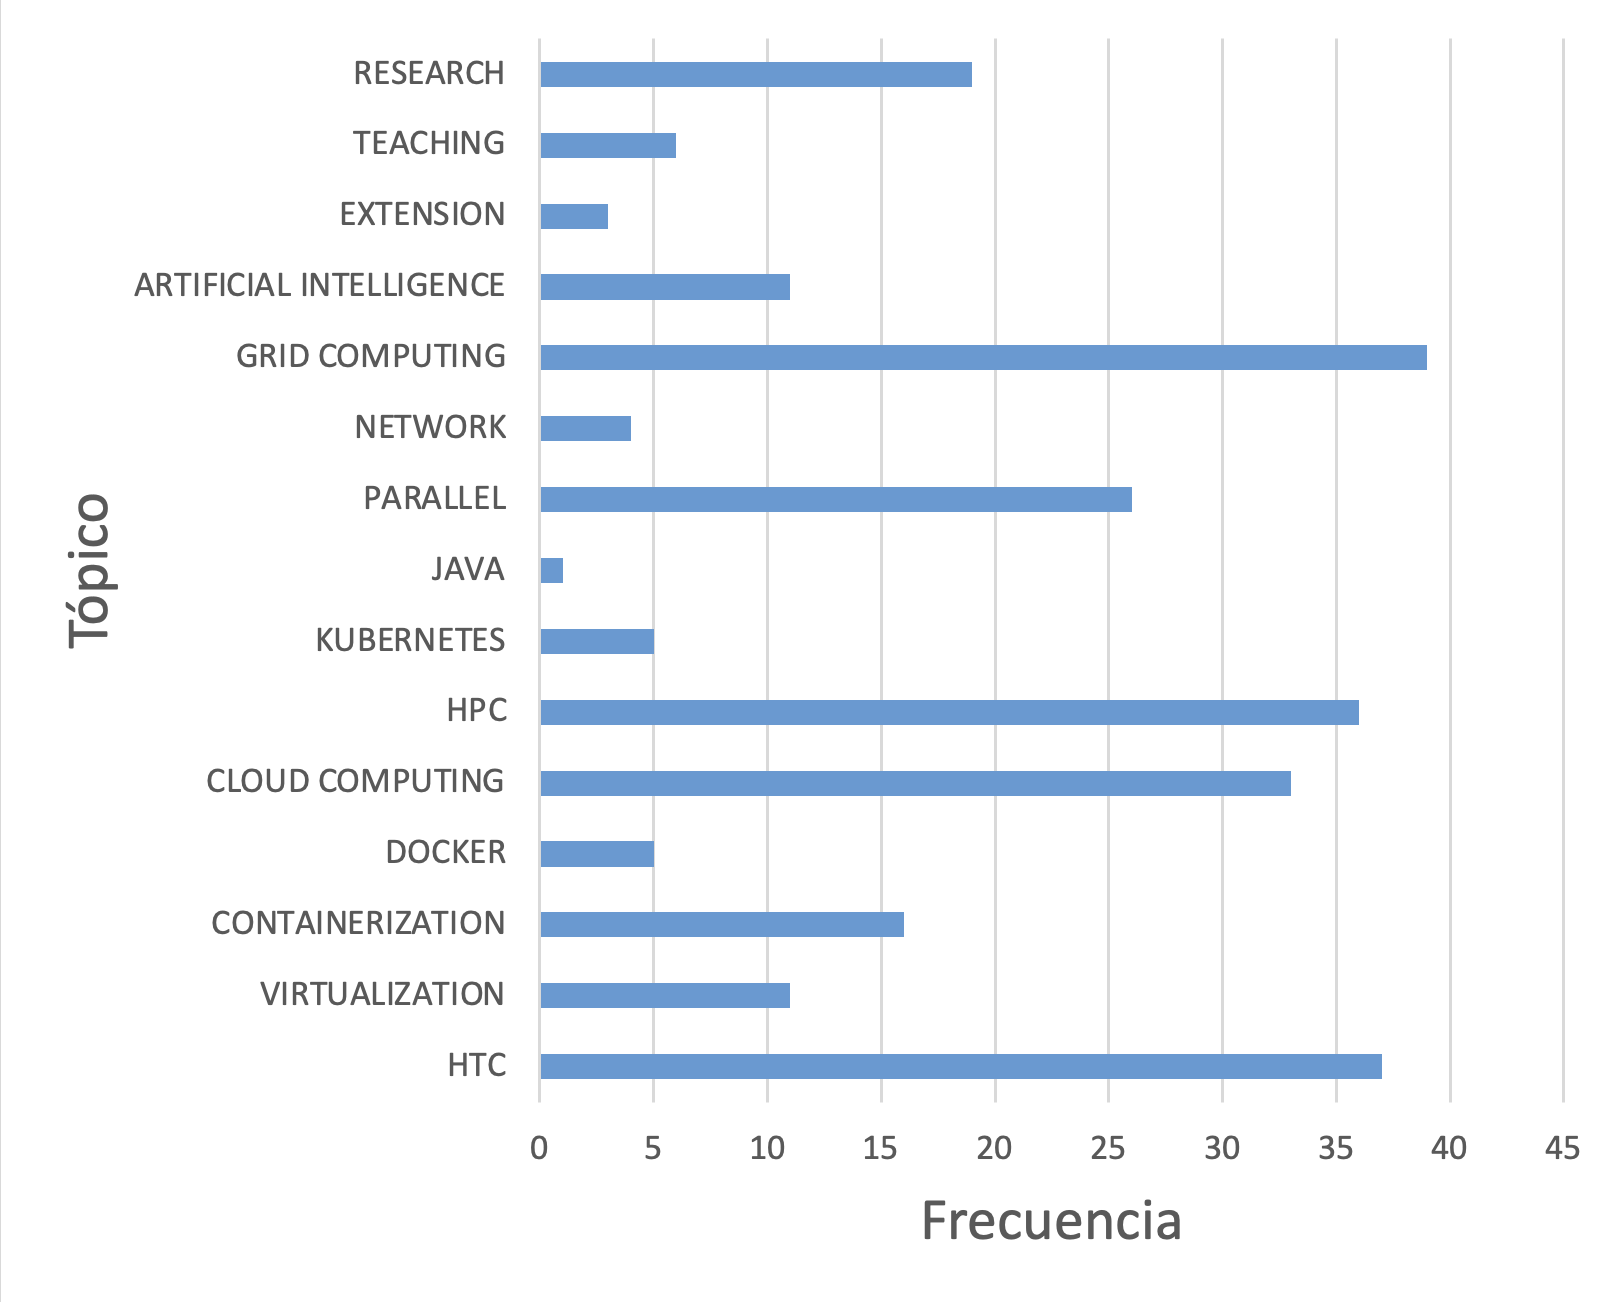
\includegraphics[scale=0.3] {tablas-images/sms/plot-topicos.png}
	\caption{Diagrama del proceso de eliminación de resultados}\label{fig:plot-topicos}
\end{figure}


\subsection{Conformidad con las preguntas de investigación}
Respecto al Cumplimiento con las preguntas de investigación (RQ) planteadas en la sección \ref{subsubsec:RQ-def}, todos los 114 estudios cumplían con la \textbf{RQ1}, mientras que únicamente 28 de estos cumplían con la \textbf{RQ2}. Ver figura \ref{fig:plot-venn-RQs}

\begin{figure}[H]
	\centering
	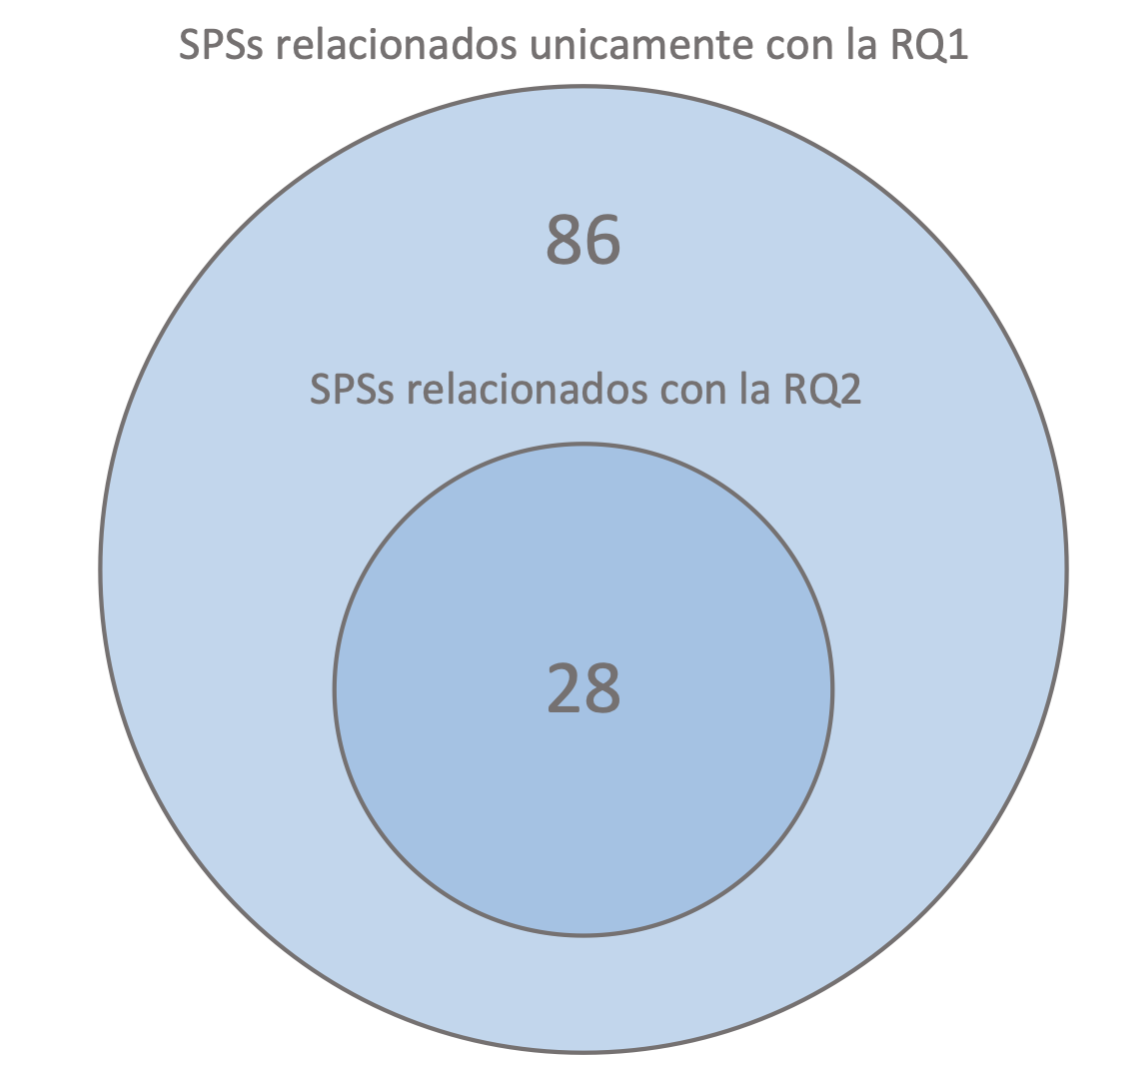
\includegraphics[scale=0.3] {tablas-images/sms/plot-venn-RQs.png}
	\caption{Diagrama del proceso de eliminación de resultados}\label{fig:plot-venn-RQs}
\end{figure}



\section{Información de la herramienta}

\noindent
La herramienta utilizada para este proceso de revisión de la literatura fue \textbf{SMS-BUILDER}, desarrollada por el Dr. Christian Andres Candela Uribe la cual se encuentra disponible en \textit{Docker Hub}. La imagen puede consultarse en el siguiente enlace:

\begin{center}
	\href{https://hub.docker.com/r/griduq/sms-builder}{\texttt{https://hub.docker.com/r/griduq/sms-builder}}
\end{center}



\section{Reproducibilidad del método}
\noindent
Con el fin de fomentar la reproducibilidad del método de revisión, se proporcionan dos mecanismos de verificación que permiten a los revisores y lectores acceder de forma transparente a la información utilizada, generada mediante la herramienta SMS-Builder de~\cite{SMSBuilder2020}
\begin{itemize}
	\item Un enlace de acceso público a la instancia de SMS-Builder que contiene todos los datos del proceso de revisión sistemática: \href{https://sms-htcondor.iti.grid.uniquindio.edu.co}{link}. Las credenciales de acceso son ``invitado'' tanto para el nombre de usuario como para la contraseña.
	\item Una imagen de Docker de acceso público que integra toda la documentación necesaria para crear un contenedor con los datos del proceso: \href{https://hub.docker.com/r/parritap/sms-htcondor-universes}{link}.
\end{itemize}

\noindent
Adicionalmente, se implementaron procesos de respaldo como medida de seguridad. Estos \textit{backups} fueron almacenados en ubicaciones diferentes, siguiendo la estrategia de respaldo \textbf{3--2--1}.



\section{Conclusiones de la revisión sistemática de la literatura}
\noindent
Esta revisión sistemática de la literatura sobre universos de HTCondor y tecnologías de computación distribuida de alto rendimiento logró identificar y analizar 114 estudios relevantes de un total inicial de 847 documentos recuperados de cinco bases de datos académicas principales. El proceso metodológico incluyó la aplicación de criterios de inclusión y exclusión que redujeron el corpus inicial en un 43.44\%, seguido de la eliminación de duplicados y la aplicación de estrategias complementarias como la búsqueda por bola de nieve. Los resultados revelan que la base de datos ACM fue la fuente más productiva con el 61.16\% de los artículos iniciales, mientras que IEEE y Taylor \& Francis no proporcionaron contribuciones significativas con las cadenas de búsqueda empleadas. El análisis temático identificó como tópicos predominantes \textbf{Grid Computing, HPC, Cloud Computing, HTC y Parallel}, evidenciando una concentración de la investigación en estas áreas específicas. Respecto al cumplimiento de las preguntas de investigación, todos los 114 estudios seleccionados respondieron a RQ1 (trabajos relacionados con universos de HTCondor en diversos dominios computacionales), mientras que solo 28 estudios (24.6\%) abordaron RQ2 (aplicaciones en funciones universitarias esenciales), lo que sugiere una brecha significativa en la literatura sobre la aplicación de estas tecnologías en contextos educativos y de extensión universitaria. La distribución temporal de las publicaciones y la diversidad de métricas de calidad aplicadas confirman la relevancia y actualidad del tema de investigación, proporcionando una base sólida para el desarrollo de taxonomías y marcos de trabajo en el dominio de HTCondor y computación distribuida.
